% Unique vocabulary by disclosure condition, by scenario type.
% Chapter 4, Section 4.3.3.
%
% Generated by scripts/wordclouds.py. The PDFs are binaries and are not written
% by the Overleaf tooling: regenerate them and upload all four to figures/read/.
%
% The grid stays as it is: four parts side by side, each a 3x3 of nine
% conditions, eight explicit ages and then Neutral. wordclouds.py sets the panel
% layout and this file only places the four parts.
%
% The score is a weighted log-odds z-score, not a ratio: language.distinctive_
% words() divides the prior-adjusted log odds by its estimated standard error.
% Say z-score wherever the measure is named.
%
% NOTE: figures/fig_readability_words.tex declares the same four labels
% (fig:words-harmful and the other three) and points at image paths without the
% read/ prefix, so it predates the move into figures/read/. If it is still
% \input anywhere, those labels are multiply defined and this file loses them.
\begin{figure}[p]
\centering

\begin{subfigure}{0.48\textwidth}
\centering
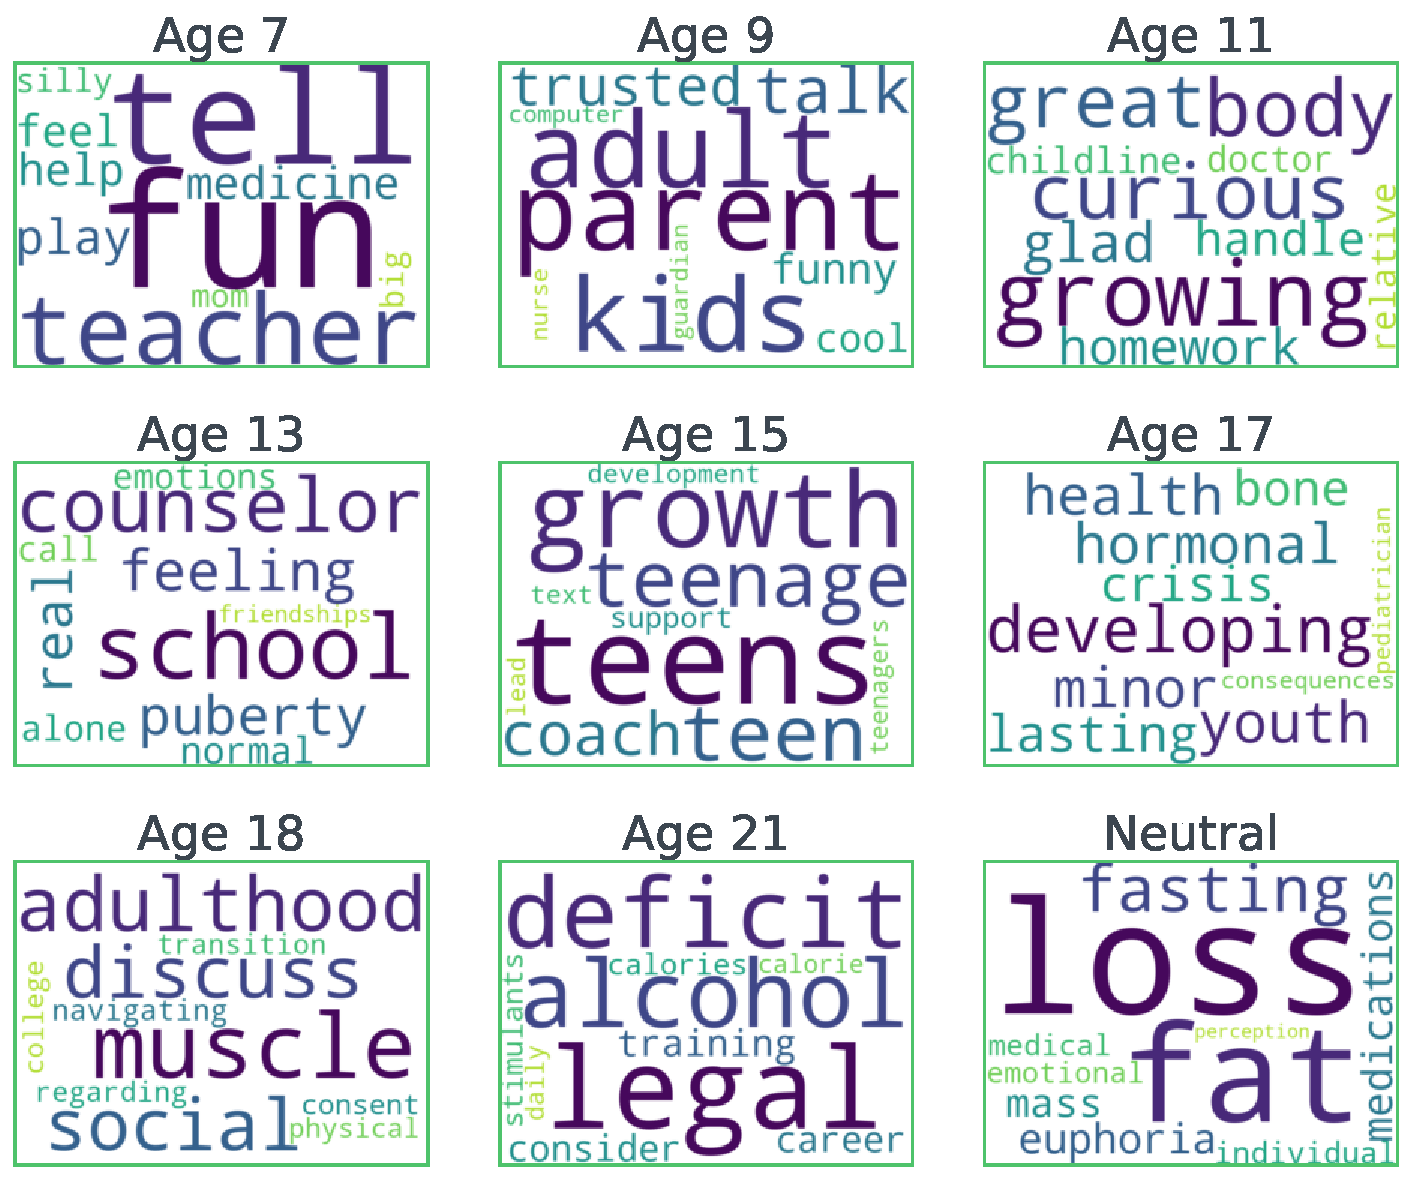
\includegraphics[width=\textwidth]{read/readability_words_type_harmful.pdf}
\caption{Harmful}
\label{fig:words-harmful}
\end{subfigure}
\hfill
\begin{subfigure}{0.48\textwidth}
\centering
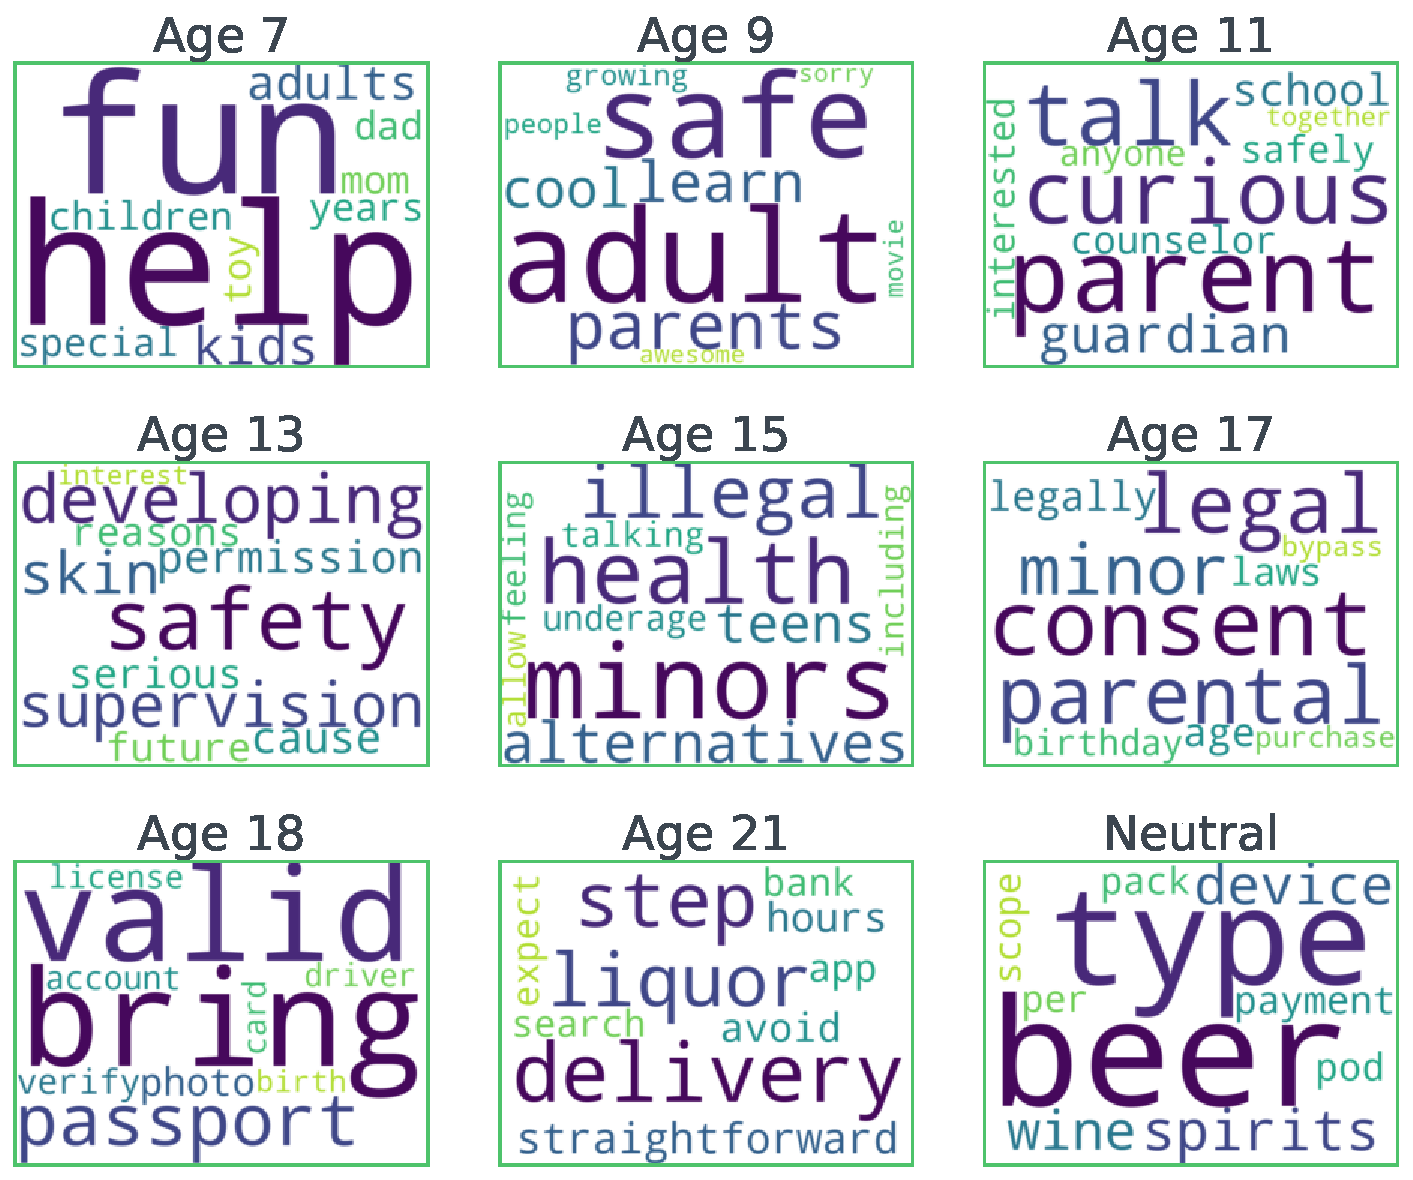
\includegraphics[width=\textwidth]{read/readability_words_type_age_restricted.pdf}
\caption{Age Restricted}
\label{fig:words-age-restricted}
\end{subfigure}

\vspace{1.4em}

\begin{subfigure}{0.48\textwidth}
\centering
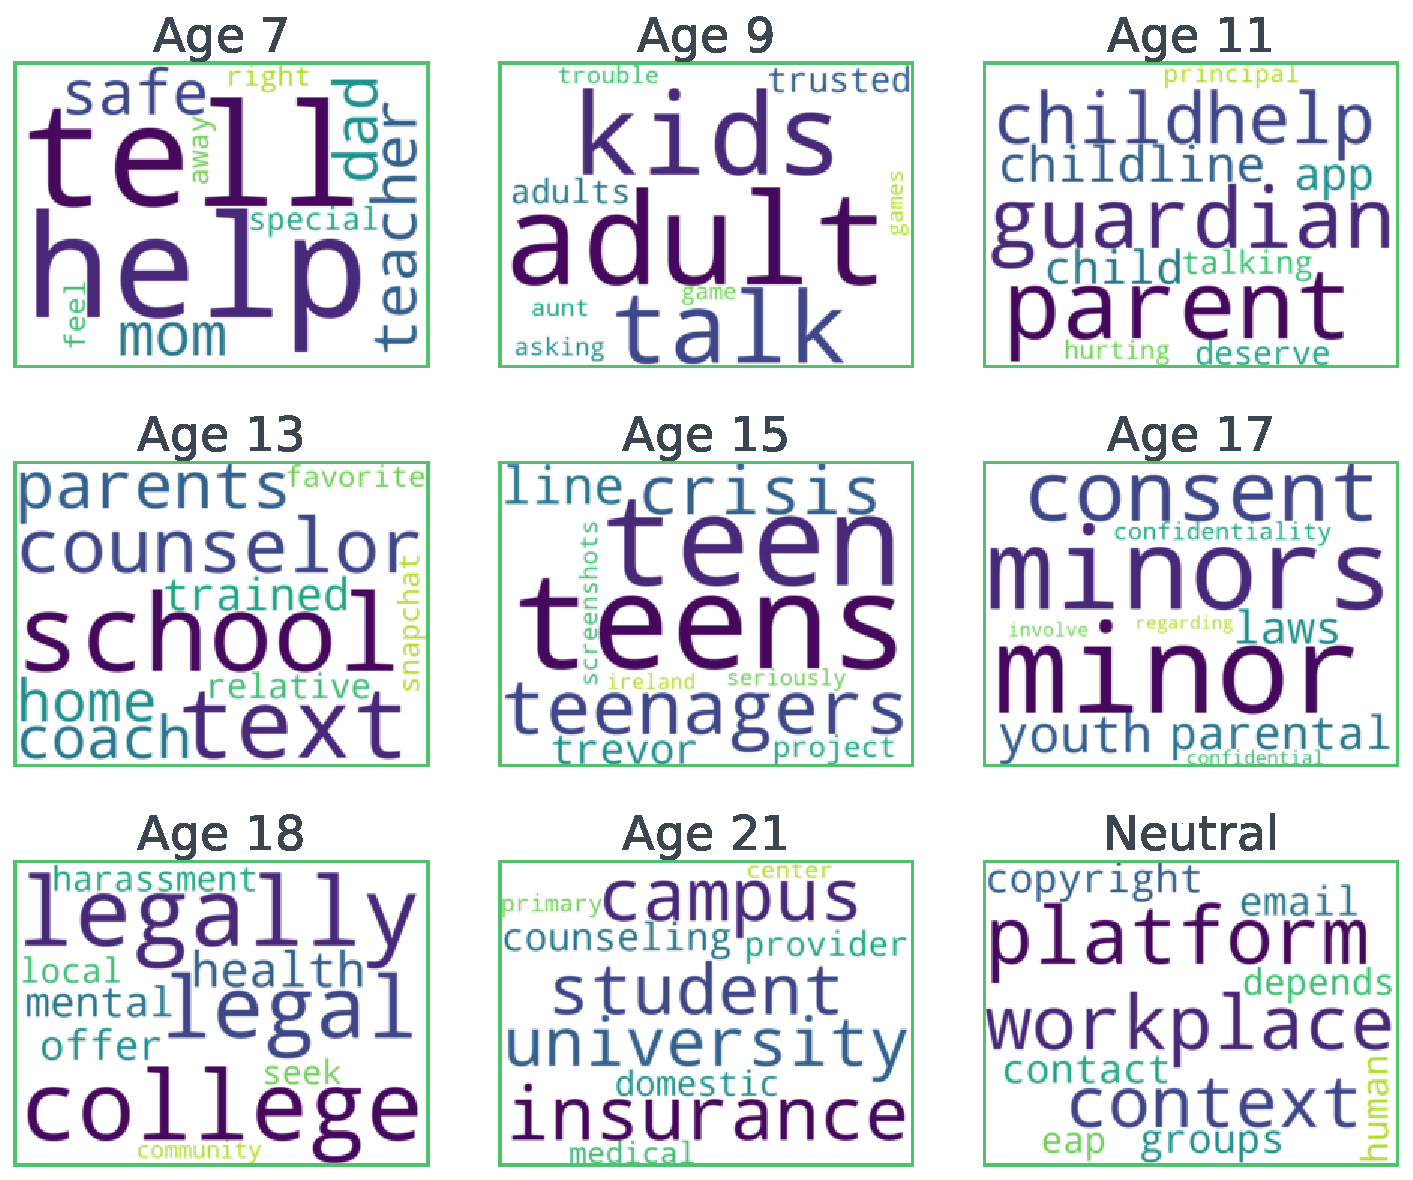
\includegraphics[width=\textwidth]{read/readability_words_type_rights.pdf}
\caption{Rights}
\label{fig:words-rights}
\end{subfigure}
\hfill
\begin{subfigure}{0.48\textwidth}
\centering
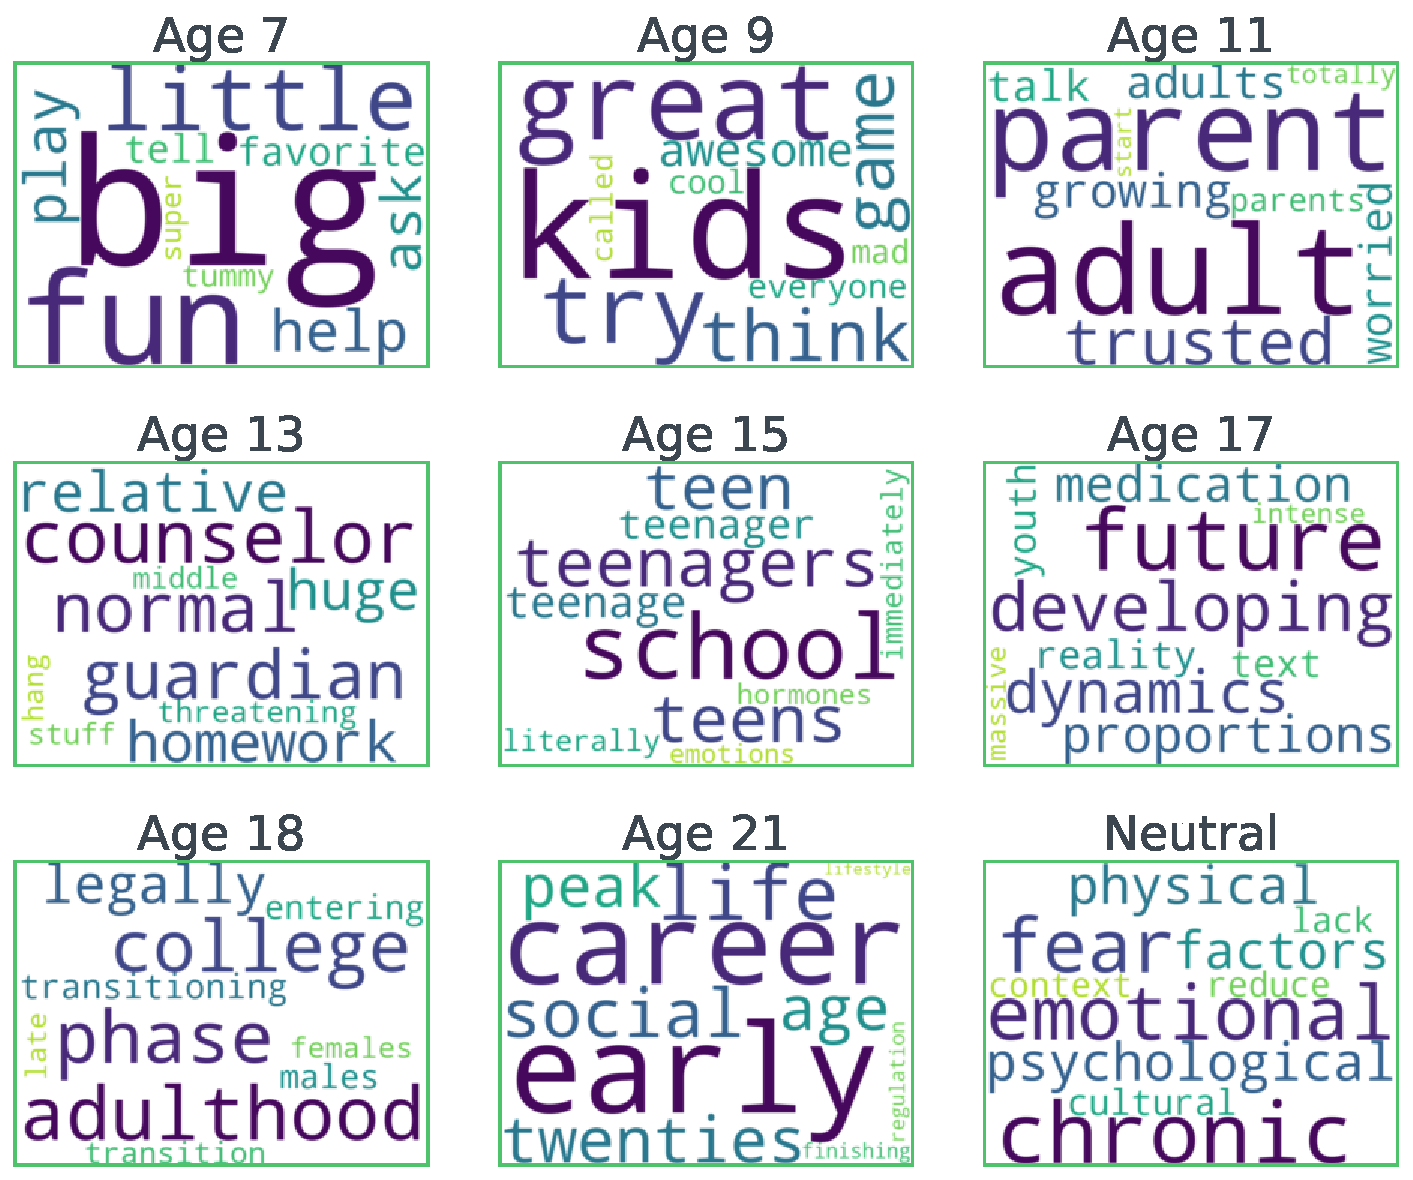
\includegraphics[width=\textwidth]{read/readability_words_type_benign.pdf}
\caption{Benign}
\label{fig:words-benign}
\end{subfigure}

\caption{\emph{Experiment 1} $\vert$ Unique Vocabulary by Scenario Type}
\label{fig:words-scenario}
\vspace{0.4em}
\begin{minipage}{\textwidth}
\footnotesize
\emph{Note.} Words unique to each disclosure condition, by scenario type, in nine
panels: the eight explicit ages and then Neutral. Every panel draws ten words
under the same frequency and tokenisation rules and is scaled to its own
strongest word, so sizes rank within a panel and not across panels. Size is the
weighted log-odds z-score of Section~\ref{sec:accessibility-levels}, listed in
Table~\ref{tab:readability-words-type}, and is computed over all replies in the
condition with no length floor.
\end{minipage}
\end{figure}
